\subsection{Shared L2 Cache}
The L2 cache is shared by and coherent with all the L1 I/D caches.
The coherence protocol is a 4-hop MESI protocol based on the thesis of Vijayaraghavan~\cite{murali}.
It also provides an coherent-access interface for memory accesses that are not sent by the L1 caches.
For example, the coherent-access interface can be used for performing page walks in the L2 TLBs of each core.
It can also be used to initialize the memory contents while the processor is starting up.

\subsubsection{Interface}

\begin{figure}
\begin{lstlisting}[caption={}]
interface LLCache;
  interface ParentCacheToChild#(LLCRqId, LLChild) to_child;
  interface DmaServer#(LLCDmaReqId) dma;
  interface MemFifoClient#(LdMemRqId#(LLCRqMshrIdx), void) to_mem;
  interface Perf#(LLCPerfType) perf;
endinterface
module mkLLCache(LLCache);
  // implementation
endmodule
\end{lstlisting}
\caption{Interface of L2 cache}\label{fig:l2-cache-ifc}
\end{figure}

Figure~\ref{fig:l2-cache-ifc} shows the interface of the L2 cache:
\begin{itemize}
    \item Subinterface \code{to\_child}: contains FIFO interfaces connected to the L1 caches.
    Type \code{LLChild} is to identify the L1 cache, while type \code{LLCRqId} is to identify the request from a given L1 cache.
    \item Subinterface \code{dma}: contains FIFO interfaces to perform coherent accesses on the memory system.
    As shown in Figure~\ref{fig:uncore}, the L2 TLBs and the memory loader use this port to read and write the memory system.
    \item Subinterface \code{to\_mem}: contains a pair of FIFO interfaces to send requests to DRAM and receive responses from DRAM, respectively.
    \item Subinterface \code{perf}: is for querying performance counters. 
\end{itemize}

\subsubsection{Implementation}

\begin{figure}
    \centering
    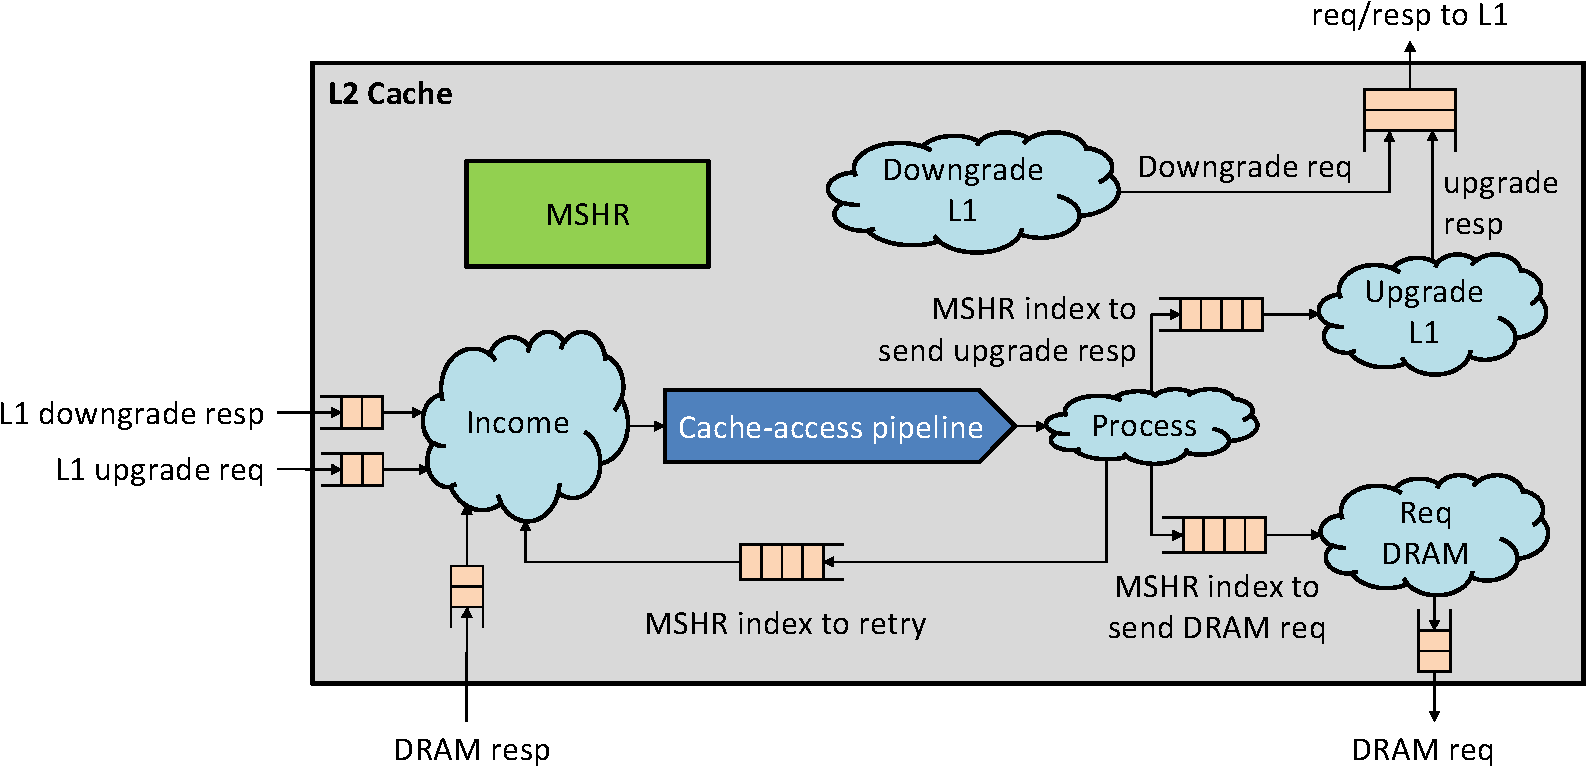
\includegraphics[width=\columnwidth]{fig/l2_cache_crop.pdf}
    \caption{Implementation of L2 cache}\label{fig:l2-cache-impl}
\end{figure}

Figure~\ref{fig:l2-cache-impl} shows the internal implementation of the L2 cache.
It is very similar to the implementation of the L1 cache (Section~\ref{sec:d-cache}).
All incoming messages to the L2 cache are first processed by the Income rules which enter the messages to the cache-access pipeline.
At the end of the pipeline, the Process rules process these messages.
The Process rules may send responses to L1s, send requests to DRAM, and wake up requests in MSHR.
The difference is the addition of the Downgrade-L1 rule, which scans MSHRs for requests that need to downgrade L1s and sends downgrade requests to L1 caches.

\subsubsection{Source Code}
See the followings:
\begin{itemize}
    \item module \code{mkLLCache} in \code{//procs/lib/LLCache.bsv}, and
    \item module \code{mkLLBank} in \code{//coherence/src/LLBank.bsv}.
\end{itemize}
